
\documentclass{article}
\usepackage{mathtools}
\usepackage{graphicx}
\usepackage{subcaption}
\title{Assignment 1}
\date{August 28, 2020}
\author{Haixiang Zhu}
\begin{document}
\maketitle
\begin{enumerate}
	\item 
    \begin{enumerate}
    	\item  The steay state condition:
    	\begin{align*}
		  &\Delta k = sy-\delta k = 0\\
		  \Rightarrow&0.3k^{\frac{1}{2}}=0.1k\\
		  \Rightarrow&
		  \begin{cases}
			k^\ast=9\\
			y^\ast=(k^\ast)^{\frac{1}{2}}=3\\
			i^\ast=\delta k^\ast=0.9\\
			c^\ast=y^\ast-i^\ast=2.1
		  \end{cases}
		\end{align*}
		\begin{figure}[h!]
			\centering
		  	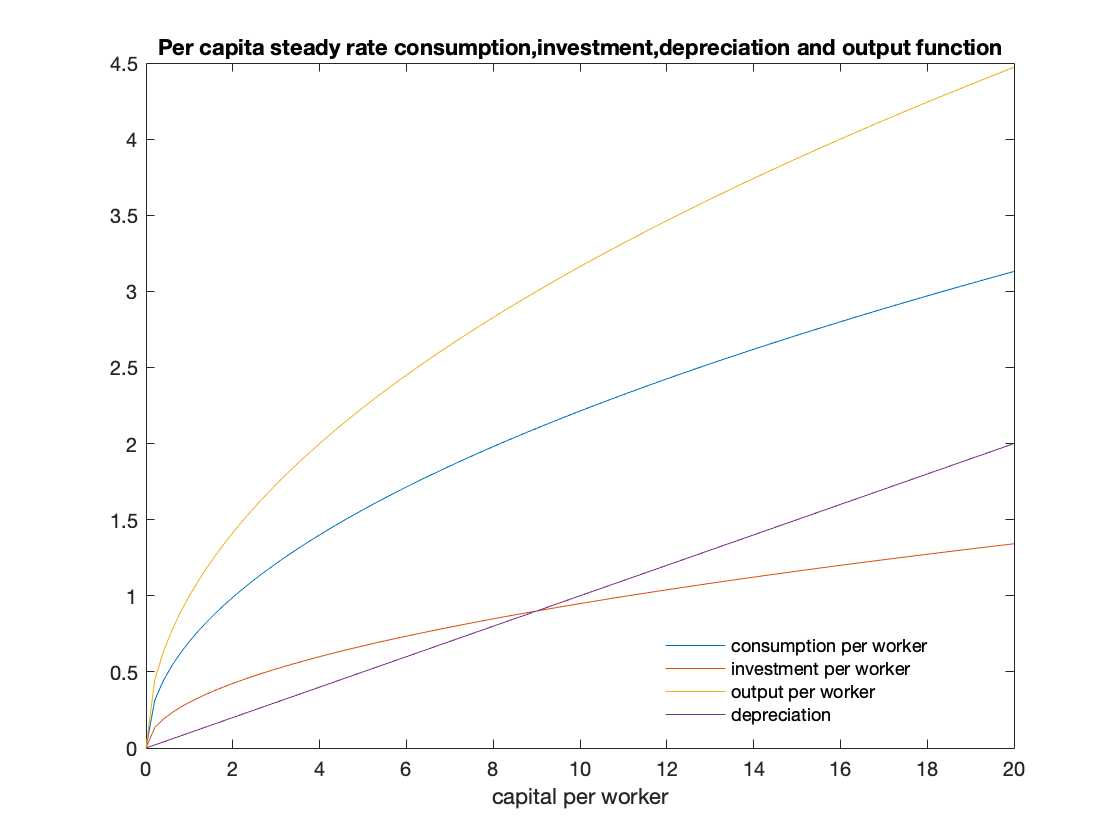
\includegraphics[width=.99\linewidth]{1_1a.png}
		  	\caption{The steady state of Solow Model}
		\end{figure}
		\newpage
        \item The MATLAB code is in attached file ``solow\_1\_bc.m''.
        \begin{figure}[h!]
		  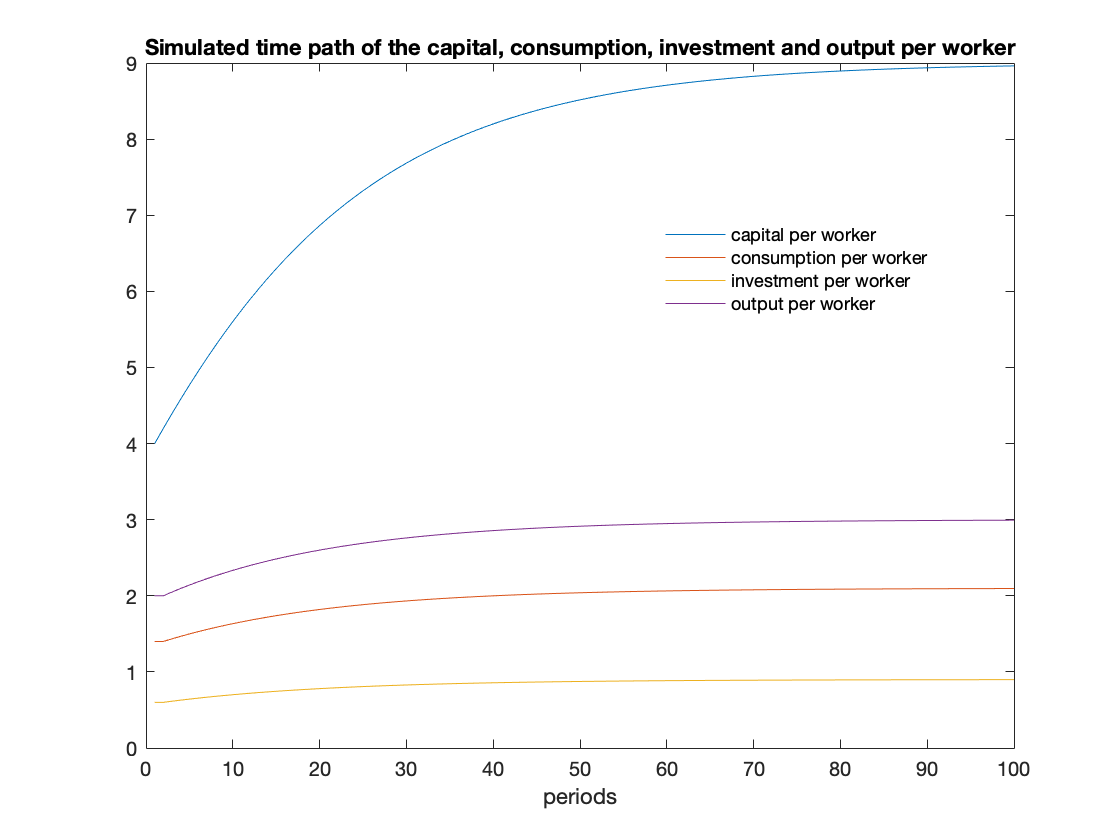
\includegraphics[width=\linewidth]{1_1b.png}
		  \caption{Simulation of Solow Model with $k_0$=4}
		\end{figure}
        \newpage
        \item The MATLAB code is in attached file ``solow\_1\_bc.m''.
        \begin{figure}[h!]
		  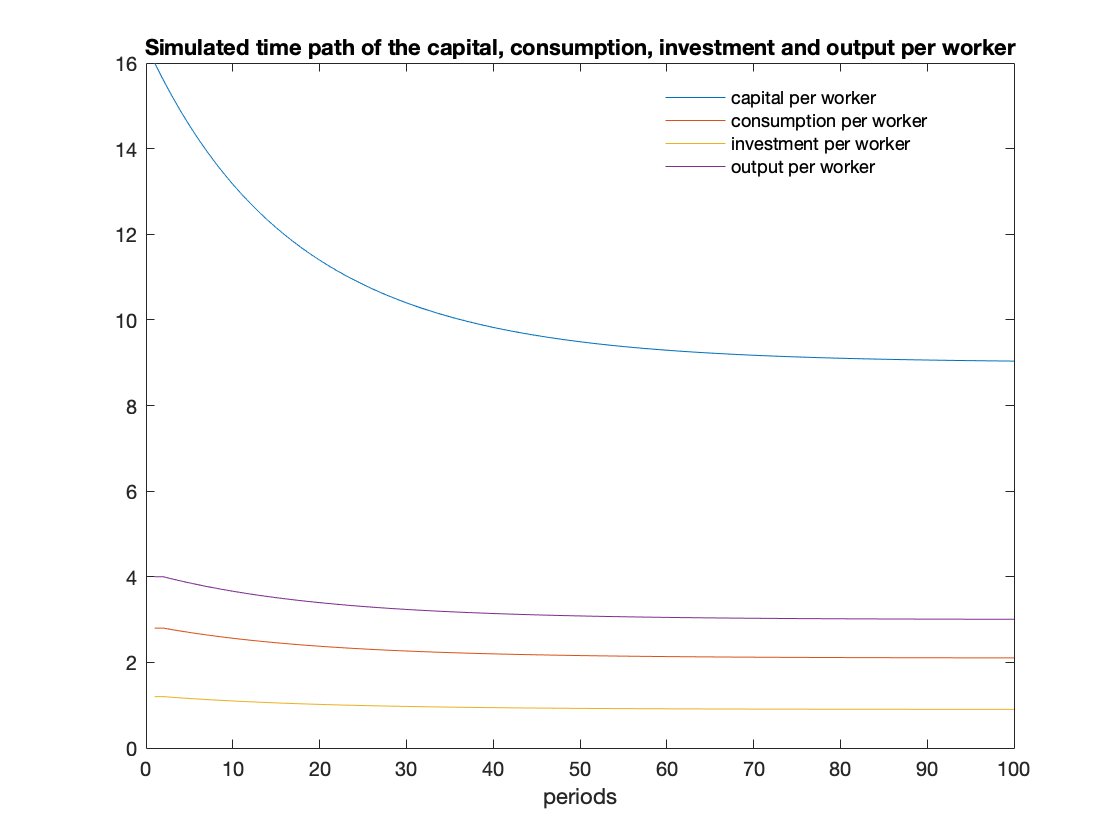
\includegraphics[width=\linewidth]{1_1c.png}
		  \caption{Simulation of Solow Model with $k_0$=16}
		\end{figure}
        \item At the steady state of this economy:
		\begin{align*}
        	&\begin{dcases}\frac iy=\frac{\delta k}y=\frac{sy}y=0.08\\\frac ky=2.5\end{dcases}\\
        	\Rightarrow&
		 	\begin{dcases}s^\ast=0.08\\\delta^\ast=0.032\end{dcases}
        \end{align*}
    \end{enumerate}
    \item 
    \begin{enumerate}
    	\item The MATLAB code is in attached file ``solow\_2\_abc.m''.\\
    	With the number of samples N =1000,\\
	    an approximation of the golden rule consumption per worker = 2.499997\\
	 	an approximation of the golden rule savings rate =  0.499499\\
	 	an approximation of the golden rule capital per worker =  24.949975\\
	    \newpage
	    \item The MATLAB code is in attached file ``solow\_2\_abc.m''.
	    \begin{figure}[h!]
			  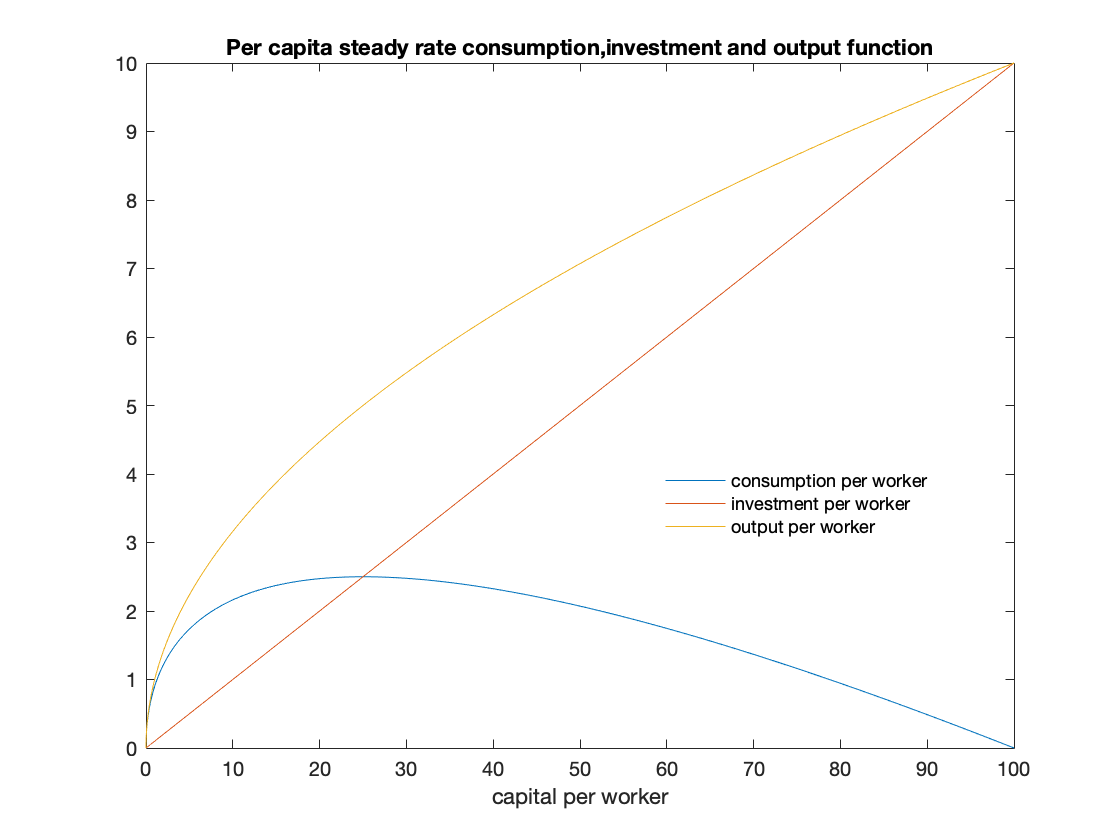
\includegraphics[width=\linewidth]{1_2b.png}
			  \caption{The steady state of Solow Model}
			\end{figure}
		\newpage
		\item The MATLAB code is in attached file ``solow\_2\_abc.m''.
	    \begin{figure}[h!]
			  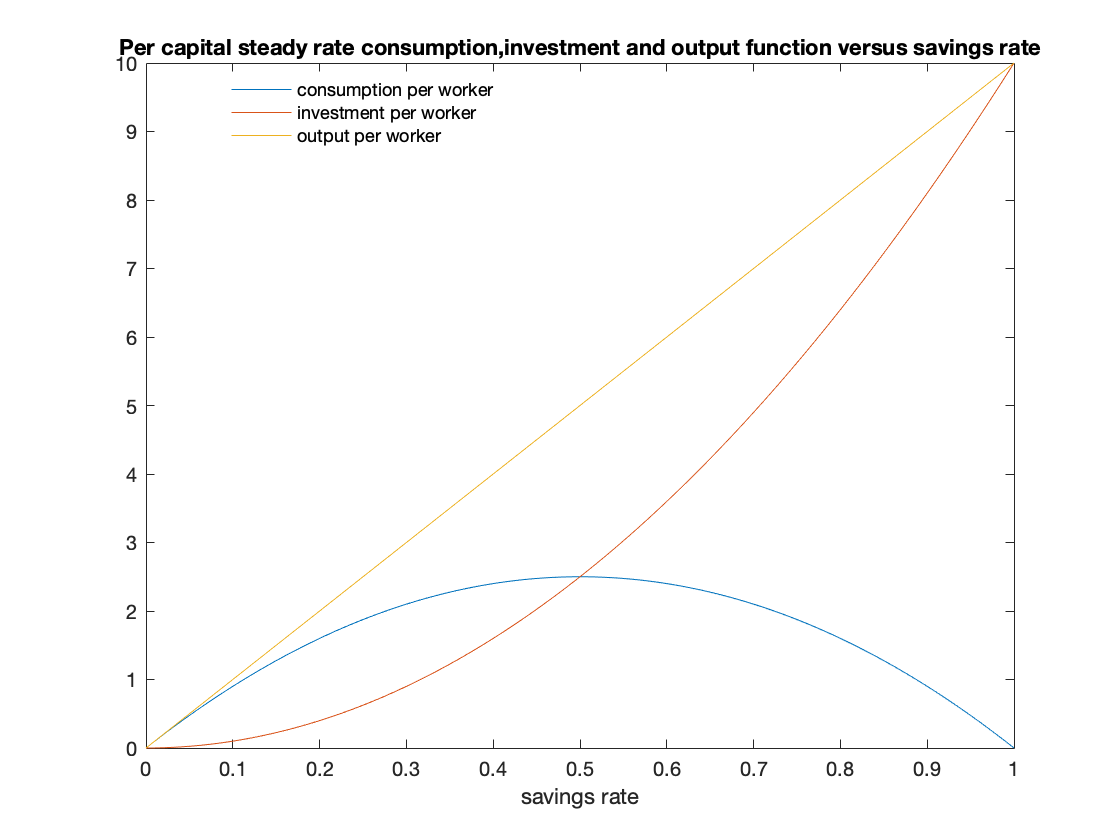
\includegraphics[width=\linewidth]{1_2c.png}
			  \caption{The steady state of Solow Model}
			\end{figure}
		\item According to Golden Rule:
	    \begin{align*}
	    &{y}'=\delta\\
	    \Rightarrow&\frac12k^{-\frac12}=0.1\\
	    \Rightarrow&\begin{cases}k_{gold}=25\\y_{gold}=5\\i_{gold}=2.5\\c_{gold}=2.5\end{cases}\\
	    \Rightarrow &s_{gold}=\frac{i_{gold}}{y_{gold}}=0.5
		\end{align*}
	    which is aligned with the numerical results in part(a).
    \end{enumerate}
    \item According to Golden Rule:
    \begin{align*}
    &{y}'=\delta\\
    \Rightarrow&\alpha k^{\alpha-1}=\delta\\
    \Rightarrow&k^{1-\alpha}=\frac\alpha\delta\\
    \Rightarrow&s=\frac{\delta k}y=\frac{\delta k}{k^\alpha}\\
    \Rightarrow&s=\delta k^{1-\alpha}=\delta\cdot\frac\alpha\delta=\alpha
	\end{align*}
\end{enumerate}
\end{document}